\section{Methods}

We seek to extend the method of \cite{zhao2011large} to deep convolutional
neural networks.  We show that by using soft labels, our model can achieve
better classification performance.

% In addition, we also see if soft labels can
% help reduce the required number of training examples.

%Based on the work of
%\cite{hinton2015distilling}, we will see if we can reduce the architectural
%complexity of our network (thus reducing training and evaluation time).

We compare different schemes for obtaining soft labels for ImageNet
categories.  In doing so, we explore semantic similarity measures derived from
word embeddings trained on large amounts of text, knowledge bases such as 
WordNet, as well as visual similarity metrics and compare them against each
other.


\subsection{Soft Labels}
\label{sec:soft_labels}

\begin{table}[!tb]
  \centering
  \begin{tabular}{|c|c|c|c|c|c|}
    \hline
      & Sax & Limo & Church & Yurt & Obelisk \\
    \hline
      \textbf{1-hot} & 1 & 0 & 0 & 0  & 0 \\
    \hline
      \textbf{Soft} & 1 & 0.5 & 0.14 & 0.43 & 0.43 \\
    \hline
  \end{tabular}
  \caption{
    A \emph{1-hot label} vector vs. a \emph{soft label} vector for
    ``saxophone'' among 5 classes.
  }
  \label{tbl:soft_labels}
\end{table}

Traditionally when training a classifier, the loss function would be computed
by comparing the prediction values against a 1-hot label vector.
A 1-hot label means that the correct (ground truth) category is given a value
of 1 and all other categories are given a value of 0.
When the classifier makes an error, it is not given any ``partial credit''
based on the semantic relevance of its mistake.

On the contrary, soft labels provide a real-valued distribution over
the object categories. Thus, the classifier is not penalized as
heavily for making a semantically relevant error (e.g. misclassifying
a ``donkey'' as a ``mule'') as it would be for a completely incorrect
prediction (e.g. misclassifying a ``truck'' as a ``cat''). The use of
soft labels also encourages assigning a small amount of probability
mass to semantically-related classes. A model which is able to assign
probability mass to semantically-related classes consequently has a richer
understanding of the image than a model which assigns high probability mass to
unrelated classes. An example is shown in Table \ref{tbl:soft_labels}.
Note that the identity is always kept at 1; that is, a class is always
100\% similar to itself.

A soft labeling scheme can be visualized by an \emph{affinity matrix}. Figure
\ref{fig:aff-5_1} shows a five class affinity matrix. For affinity matrix $A$,
element $A_{ij}$ is the similarity (i.e. \emph{affinity}) between class $i$ and
class $j$. Affinity matrices are typically symmetric (i.e. $A_{ij} = A_{ji}$ for
all $i, j$), although we violate this constraint word2vec similarity scheme (for
an example see Section \ref{word2vec}).

\begin{figure}[!tb]
%\begin{figure}[t]
  \centering
  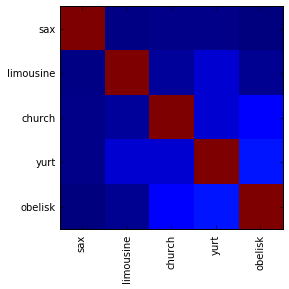
\includegraphics[width=0.4\textwidth]{figs/aff-5_1.png}
  \caption{
      Affinity matrix for five ImageNet classes computed from word2vec word
      similarity. Note that \emph{church}, \emph{yurt}, and
      \emph{obelisk} have high similarity, due to their building nature, while
      \emph{limousine} and \emph{sax} have low similarity to most other classes.
  }
  \label{fig:aff-5_1}
\end{figure}

\subsection{Linguistic Semantic Similarity}


\subsubsection{WordNet}

WordNet is a large database of English words grouped into synonym sets called
sysnets \cite{miller1995wordnet}.
The sysnets are related hierarchically with semantic and conceptual links, such
as hypernyms (``is a'') and meronyms (``part of'') relationships.

Using the distance metric in equation \ref{eq:wordnet_dist}, we follow the work
of \cite{fergus2010semantic} and \cite{zhao2011large} for defining soft labels
for a deep CNN classifier. We experimentally test a wide variety of
hyperparameters and values for $\kappa$, which measures how diffuse or sparse
the similarity distribution is. We find that values between 3 and 7 work best.

We use three different similarity metrics between hypernyms in WordNet.
First, we use equation \ref{eq:wordnet_dist} as defined in \cite{zhao2011large}.
We also use the WUP distance metric (as defined in
\cite{budanitsky2006evaluating}) and the PATH distance metric:
\begin{equation}
\label{eq:path_dist}
\mathrm{PATH}(\mathrm{label}_i, \mathrm{label}_j) =
  \frac{1}{\mathrm{path\_len}(\mathrm{label}_i, \mathrm{label}_j)}
\end{equation}
In general, we found that equations \ref{eq:wordnet_dist} and \ref{eq:path_dist}
work best.


\subsubsection{Word Embeddings} \label{word2vec}

A word embedding maps each word in a lexicon to a continuous
real-valued vector. This nature of this mapping is often guided by the
distributional hypothesis introduced in
\cite{harris1954distributional}, which states that a word can be
understood by the context it appears in. Assuming this hypothesis, a
desirable mapping is one that maps words which appear in similar
contexts to nearby locations in the vector space.

Popular methods for computing word embeddings such as word2vec
\cite{mikolov2013distributed} and GloVe \cite{pennington2014glove} have been
shown to capture such properties.  However, \cite{levy2014dependency} shows that
when context is varied, the notion of similarity between words also changes. For
example, when context is taken to be neighboring words, words close in the
vector space tend to be \emph{topically} similar. Conversely, when context is
defined via \emph{linguistic dependencies}, nearby words tend to be
\emph{semantically} similar. We examine the effect word context has on semantic
label sharing for image classification.

We construct an affinity matrix $A$ using word vectors as follows: we set the
main diagonal of the affinity matrix to 1 (i.e. $A_{ii}$ = 1 for all $i$). For
the off diagonals, we set $A_{ij}$ to be the cosine similarity between the word
vectors corresponding to label $i$ and label $j$. We perform the additional step
of applying the scaling procedure and normalization procedure to $A$: for each
row of $A$, we apply the scaling procedure of \cite{zhao2011large} to all the
elements with the main diagonal element removed and normalize these values to
sum to $s$, where $s$ is a hyperparameter. We found a value of $s = 0.5$ to work
well.  We performed this additional scaling and normalization procedure because
simply applying the scaling procedure of \cite{zhao2011large} to the each row
(i.e.  including the main diagonal element) resulted in relatively equal
probability mass for each off-diagonal entry of $A$. Additionally, each of these
off-diagonal probability masses were near-zero, hence normalizing them to sum up
to 0.5 prevents perpetually negative gradient signals for off-diagonal classes.

A side effect of this scaling and normalization procedure to each row of the
affinity matrix is that $A$ is no longer symmetric. This is illustrated in
Figure \ref{fig:aff-5_1}. For the most part we observe $A_{ij} \approx A_{ji}$.
The most drastic asymmetries occur when class $i$ is uniformly similar to all
classes and class $j$ has high similarity with one or two classes. For example,
\emph{sax} has relatively uniform similarity to all other classes, while
\emph{yurt} has high similarity for \emph{church} and \emph{obelisk} and
near-zero similarity to to \emph{sax}.

\subsection{Visual Similarity}

A main focus of our work is to exploit information embedded in natural language
to aid in visual classification.  However, it has been shown that lingustic
semantics do not always work well in modeling visual similarity
\cite{li2010building}. As an example given in \cite{li2010building}, WordNet
does not capture the correlation between ``tower'' and ``business district''.
To this end, we explore soft labeling schemes based on visual similarity
and compare the performance and label distributions to those of the lingustic
schemes.

% By better understanding the relationship between linguistic similarity
% and the visual representations learned by a CNN, we hope to explore improved
% ways of defining and weighting soft labels.  We use several existing
% methods to compute the similarities between different image categories.

We take the average GIST descriptor \cite{oliva2001modeling} values for each
category across all images in the training data set. We then use the scaled
similarity between these descriptors as a distribution across the soft labels.
Since GIST is a global descriptor, we expect it to capture more of the
background contextual information rather than similarities between the objects
themselves.


\subsection{Random Soft Labels}

As a ``sanity check'' that our method is actually working, we also train the
CNN on a randomly-generated soft label distribution. For the affinity matrix
$A$, each non-diagonal entry $A_{ij}, i \neq j$ is a randomly-generated value
between 0 and 0.25. The diagonal (identity) values are fixed at 1 as in the
other soft label schemes. We generate several random affinity matrices in this
manner and take the average score for each data set.

%To better represent the categories directly, we can also experiment with
%visual word clusters mined from images of different object categories.
%We expect that clustering SIFT descriptors \cite{lowe1999object} should work
%reasonably well.
%The similarity metric can be defined as the distance between the cluster
%centroids into which the images of different categories fall.
%We can also explore using visual vocabulary trees, introduced by
%\cite{nister2006scalable}.
%
%We can investigate many other methods. The most notable and relevant to our
%work is \cite{li2010building}, who have successfully used their visual
%similarity approach for improving hierarchical image classification.
%We can also explore other works in unsupervised clustering, including most
%recent advancements using deep neural networks in unsupervised visual
%clustering
%(Jianwei Yang, Devi Parikh, and Dhruv Batra, 2016 - not yet published).

% Possibly the trained experts thing?
